% =====================================================================
%  DSP Assignment 2 — FIR Filters
%  Group report (one submission). Lives in report/ inside the repo.
%  Compiles from report/ or from the repo root (e.g. on Overleaf).
% =====================================================================
\documentclass[11pt,a4paper]{article}

% ---------- Packages ----------
\usepackage[margin=2.3cm]{geometry}
\usepackage[T1]{fontenc}
\usepackage{lmodern}
\usepackage{textcomp}
\usepackage{amsmath,amssymb}
\usepackage{siunitx}
\usepackage{graphicx}
\usepackage{tikz}
\usepackage[section]{placeins}  % keeps figures inside their own section
\usepackage{booktabs}
\usepackage{xcolor}
\usepackage{listings}
\usepackage[hidelinks]{hyperref}
\usepackage[nameinlink]{cleveref}

\graphicspath{{Ass2/}{../Ass2/}}
\sisetup{retain-explicit-plus}

% Let the tall ECG figures share pages with text, and top-align float pages
\renewcommand{\topfraction}{0.9}
\renewcommand{\bottomfraction}{0.8}
\renewcommand{\textfraction}{0.1}
\renewcommand{\floatpagefraction}{0.92}
\makeatletter\setlength{\@fptop}{0pt}\makeatother
\setlength{\parskip}{4pt}

% Python listings
\lstset{
  language=Python,
  basicstyle=\ttfamily\footnotesize,
  keywordstyle=\color{blue!70!black}\bfseries,
  commentstyle=\color{green!40!black}\itshape,
  stringstyle=\color{orange!70!black},
  numbers=left, numberstyle=\tiny\color{gray},
  frame=single, breaklines=true, showstringspaces=false,
  columns=fullflexible, keepspaces=true,
  literate={µ}{{\textmu}}1
}

% Text the authors still have to write themselves. Must be gone before submission
\newcommand{\fillin}[1]{\textcolor{red}{\textbf{[TO COMPLETE: #1]}}}

% Label on the annotated heartbeat
\newcommand{\wave}[4]{\node[#1,font=\small\bfseries,text=red!75!black,inner sep=2pt] at (#2,#3) {#4};}

% ---------- Title ----------
\title{\textbf{Digital Signal Processing}\\[4pt]
       Assignment 2: FIR Filters\\[2pt]
       \large ECG Filtering, Adaptive Noise Cancellation and Heartbeat Detection}
\author{%
  Patrick Connolly (2777107C)\\
  Zabiallah Azar (2893681A)}
\date{}


% =====================================================================
\begin{document}
\maketitle

% =====================================================================
\section*{Recordings and Code Structure}
\label{sec:method}

We each recorded an ECG in the lab. Patrick's recording (\texttt{ecg1.tsv}) is
the signal filtered in every task, and Zabi's (\texttt{ecg2.tsv}) provides the
matched filter template in Task 5. Column 8 of each file (counting from 0)
holds the ECG in volts, which we convert to millivolts. The sampling rate
comes from the time column.

\begin{table}[htbp]
  \centering
  \caption{Recording parameters.}
  \label{tab:recording}
  \begin{tabular}{@{}lcc@{}}
    \toprule
    & \texttt{ecg1.tsv} (Patrick) & \texttt{ecg2.tsv} (Zabi) \\
    \midrule
    Sampling rate $f_s$        & \SI{250}{\hertz} & \SI{250}{\hertz} \\
    Samples $N$                & \num{13414} & \num{6985} \\
    Duration                   & \SI{53.7}{\second} & \SI{27.9}{\second} \\
    Bin spacing $f_s/N$        & \SI{0.019}{\hertz} & \SI{0.036}{\hertz} \\
    Mean (DC offset)           & \SI{-7.05}{\milli\volt} & \SI{18.81}{\milli\volt} \\
    Mains peak                 & \SI{57.5}{\micro\volt} at \SI{50.13}{\hertz}
                               & \SI{117.7}{\micro\volt} at \SI{50.11}{\hertz} \\
    \bottomrule
  \end{tabular}
\end{table}

As asked on Moodle, design and realtime operation are kept apart.
\texttt{fir\_design.py} calculates the coefficients and \texttt{fir\_filter.py}
holds the realtime \texttt{FIRfilter} class. \texttt{ecg\_plot.py} loads the
recordings and does Task 1, and \texttt{fir\_realtime\_sim.py},
\texttt{lms\_filter.py} and \texttt{heartbeat.py} are the main programs for
Tasks 2--3, 4 and 5. The only signal processing calls we use from NumPy are
\texttt{fft}, \texttt{ifft} and \texttt{hamming}, and every bin frequency is
built by hand. All filtering goes through \texttt{FIRfilter} one sample at a
time.

% =====================================================================
\section*{Task 1: ECG in the Time and Frequency Domain}
\label{sec:task1}

\begin{figure}[htbp]
  \centering
  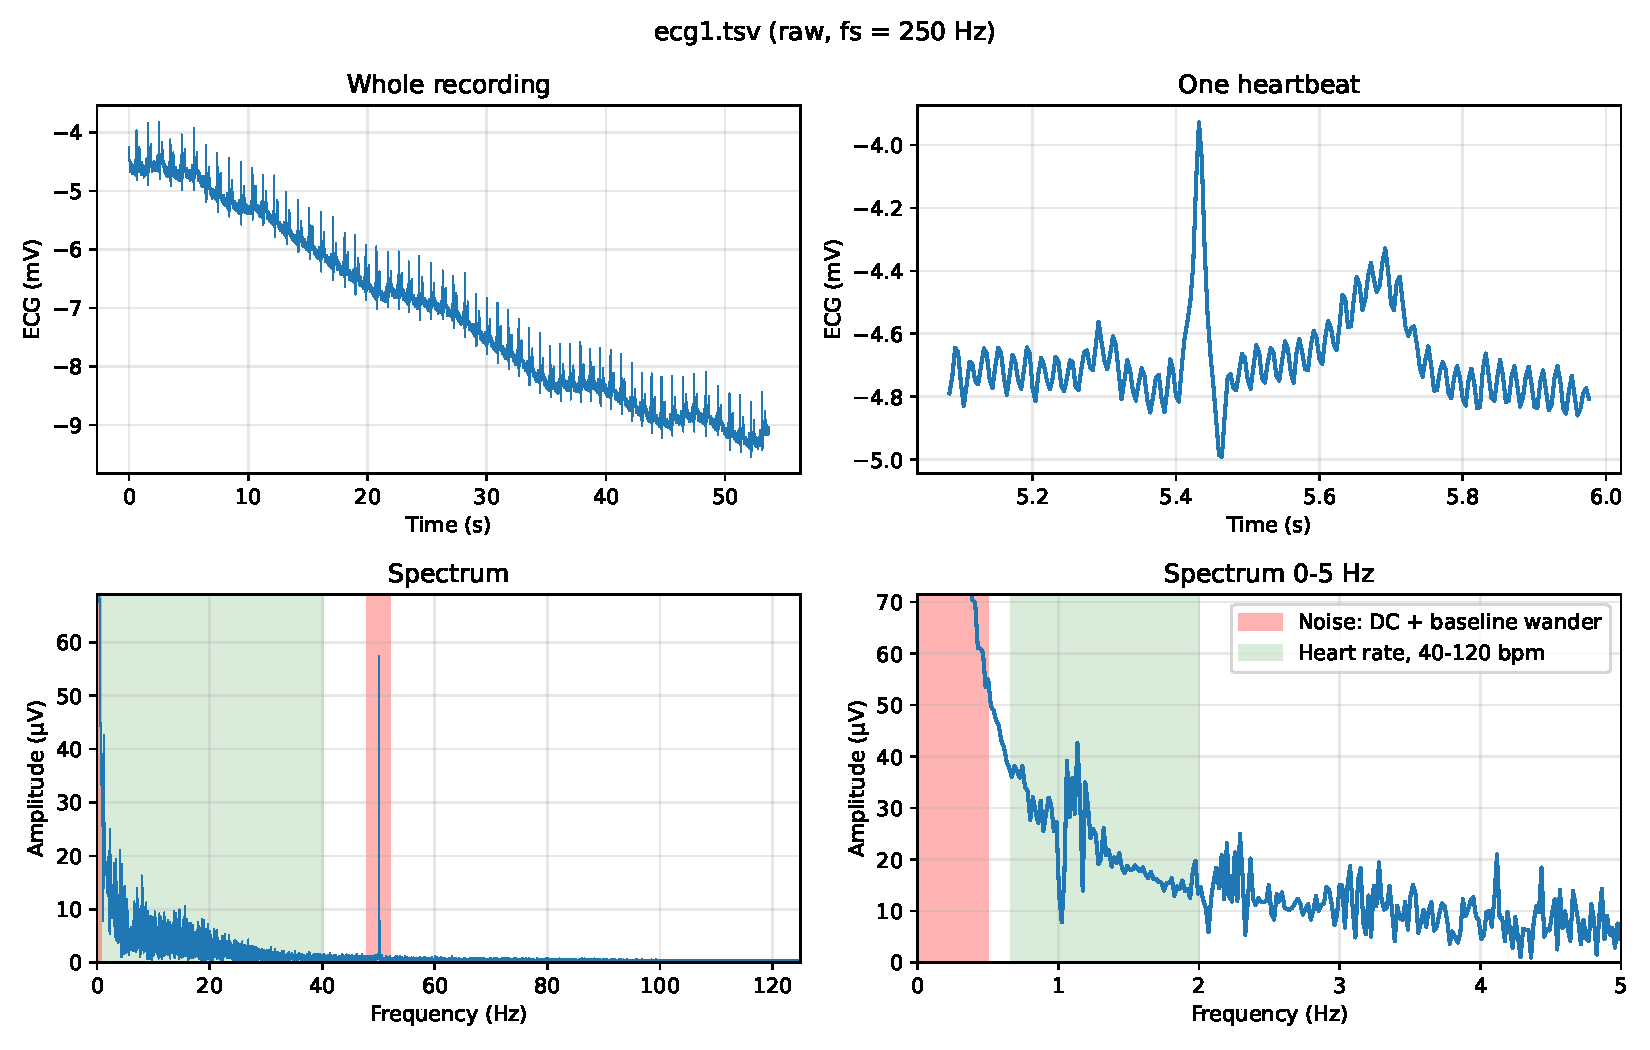
\includegraphics[width=0.97\linewidth]{ecg1_plot.pdf}
  \caption{Patrick's raw ECG (\texttt{ecg1.tsv}). Linear spectra: the bands
           kept as ECG are shaded green, those removed as noise are red.}
  \label{fig:t1_ecg1}
\end{figure}

\begin{figure}[htbp]
  \centering
  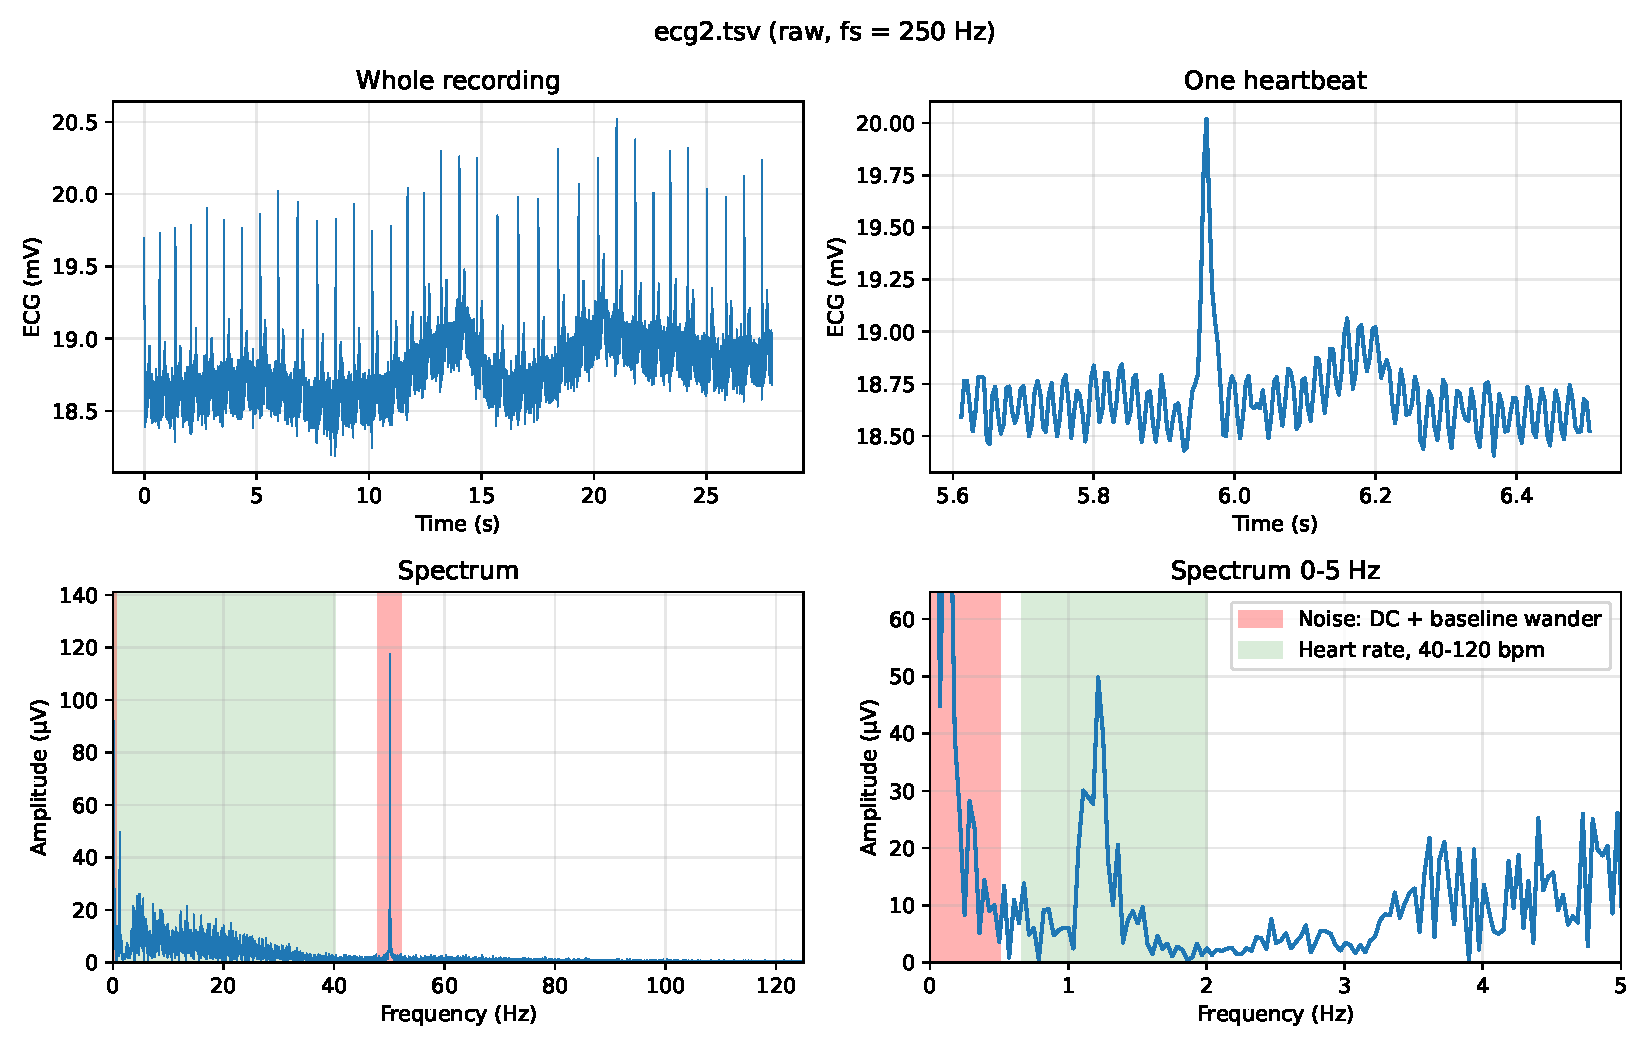
\includegraphics[width=0.97\linewidth]{ecg2_plot.pdf}
  \caption{Zabi's raw ECG (\texttt{ecg2.tsv}), shaded in the same way as
           \cref{fig:t1_ecg1}.}
  \label{fig:t1_ecg2}
\end{figure}

\paragraph{Time domain.}
The R peaks are visible in both recordings
(\cref{fig:t1_ecg1,fig:t1_ecg2}), but they sit on a large offset that drifts.
Patrick's averages \SI{-4.57}{\milli\volt} over the first second and
\SI{-9.15}{\milli\volt} over the last. A \SI{50}{\hertz} ripple runs through
both zoomed heartbeats and partly hides the P wave.

\paragraph{ECG.}
Most of the ECG lies between \SI{0.5}{\hertz} and \SI{40}{\hertz} (green). The
heart rate sets the lowest component. Zabi's shows a clear fundamental at
\SI{1.2}{\hertz}, and Patrick's is smeared over
\SIrange{0.97}{1.24}{\hertz} because Patrick's rate varies between 58 and 75 bpm
(Task 5). The largest component from \SIrange{5}{40}{\hertz} is
\SI{16.3}{\micro\volt}, falling to \SI{1.7}{\micro\volt} from
\SIrange{40}{48}{\hertz}.

\paragraph{Noise.}
\Cref{tab:noise} lists what we found in \texttt{ecg1.tsv} and what we did
about it.

\begin{table}[htbp]
  \centering
  \caption{Noise identified in the spectrum of \texttt{ecg1.tsv}.}
  \label{tab:noise}
  \begin{tabular}{@{}lll@{}}
    \toprule
    Component & Evidence & Action \\
    \midrule
    DC and baseline wander, \SIrange{0}{0.5}{\hertz}
      & up to \SI{1.75}{\milli\volt} below \SI{0.5}{\hertz}, plus the DC offset
      & remove \\
    Mains, \SIrange{48}{52}{\hertz}
      & sharp line, \SI{57.5}{\micro\volt} at \SI{50.13}{\hertz}
      & remove \\
    Mains harmonic, \SI{100}{\hertz}
      & no peak (see below)
      & leave \\
    Above \SI{52}{\hertz}
      & flat floor, at most \SI{1.3}{\micro\volt}
      & leave \\
    \bottomrule
  \end{tabular}
\end{table}

Mains harmonics lie at multiples of \SI{50}{\hertz}, but at
$f_s=\SI{250}{\hertz}$ anything above the \SI{125}{\hertz} Nyquist frequency
folds back: \SI{150}{\hertz} and \SI{350}{\hertz} land on \SI{100}{\hertz},
\SI{200}{\hertz} and \SI{300}{\hertz} land on \SI{50}{\hertz}, and
\SI{250}{\hertz} lands on DC. Every harmonic can therefore only appear at 0, 50
or \SI{100}{\hertz}, and the first two are removed anyway. In
\texttt{ecg1.tsv} there is no peak at \SI{100}{\hertz}: the largest value from
\SIrange{95}{105}{\hertz} is \SI{0.71}{\micro\volt}, at \SI{95.9}{\hertz}, so
we do not add a \SI{100}{\hertz} stop band. Zabi's recording has a faint
\SI{1.2}{\micro\volt} line at \SI{100.3}{\hertz}, \SI{40}{\decibel} below its
mains peak, which is too small to affect the template. We do not low-pass at
\SI{40}{\hertz} either, since the floor above \SI{52}{\hertz} is negligible
and a low-pass would only risk rounding the QRS complex.

% =====================================================================
\section*{Task 2: FIR Filter Design}
\label{sec:task2}

\texttt{design\_fir(fs, stop\_bands)} takes the sampling rate and a list of
(low, high) frequency ranges to remove. It follows the design steps in the
lecture notes (Sec.~6.7.8). The desired response is filled in by hand on $M$
frequency bins, with the upper half mirrored onto the lower half:
\begin{equation}
  f_k = \min(k,\,M-k)\,\frac{f_s}{M},
  \qquad
  H[k] =
  \begin{cases}
    0 & \text{if } f_k \text{ lies in any stop band,}\\
    1 & \text{otherwise,}
  \end{cases}
  \qquad k = 0,\dots,M-1.
  \label{eq:response}
\end{equation}
The IFFT of $H$ gives the impulse response with negative time in its upper
half. Swapping the halves makes it causal, and a Hamming window then smooths
the truncation to $M$ samples:
\begin{equation}
  h[n] = \mathrm{IFFT}\{H\}\!\left[\left(n-\tfrac{M-1}{2}\right)\bmod M\right]\,w[n],
  \qquad
  w[n] = 0.54 - 0.46\cos\frac{2\pi n}{M-1}.
  \label{eq:window}
\end{equation}

\paragraph{Number of coefficients.}
The IFFT samples the response every $f_s/M$\,Hz, so a stop band of width
$\Delta f$ can only be represented if $f_s/M \le \Delta f$. The narrowest band
sets the requirement, giving a minimum of $M = f_s/\Delta f_{\min}$, or 501
taps for our \SI{0.5}{\hertz} baseline band. This is only the best case,
because the window smears each band edge over a few bins. With 501 taps the
\SI{0.5}{\hertz} edge took \SI{2.3}{\decibel} off the heart rate fundamental at
\SI{1}{\hertz}, so we use twice the minimum, rounded up to the next odd number:
\begin{equation}
  M = \text{smallest odd integer} \ge \frac{2 f_s}{\Delta f_{\min}}
    = \frac{2\times 250}{0.5} \;\Rightarrow\; M = 1001.
  \label{eq:taps}
\end{equation}
The bin spacing is then \SI{0.25}{\hertz} and the gain at \SI{1}{\hertz} is
\SI{0}{\decibel}. $M$ is odd because a symmetric, odd-length filter has a
linear phase and a delay of a whole number of samples, $(M-1)/2$, while a
symmetric even-length filter is forced to zero at Nyquist, which a bandstop
cannot have. The cost is a delay of 500 samples, or \SI{2.00}{\second}. This is
set entirely by the baseline band: the \SI{4}{\hertz} wide mains band alone
would need only 125 taps.

\paragraph{Edge cases.}
A band starting at \SI{0}{\hertz} includes bin 0, because the test in
\cref{eq:response} is $f_k \ge f_\text{low}$, so DC removal needs no special
case. Windowing lets a little DC back in, but the gain at DC is only
\SI{-82.3}{\decibel}, which takes the \SI{-7.05}{\milli\volt} offset down to a
filtered mean of \SI{0.6}{\micro\volt}. An earlier version subtracted the mean
of $h$ to force the DC gain to exactly zero, but that made no practical
difference, so we removed it. Mirroring the bins in \cref{eq:response} makes
$h$ real and symmetric. Basing $M$ on the narrowest band means every band spans
at least two bins, so none can fall between them. Any number of bands can be
passed in: adding $(98, 102)$, for example, gives \SI{-51.6}{\decibel} at
\SI{100}{\hertz} with no change to the code.

\begin{figure}[htbp]
  \centering
  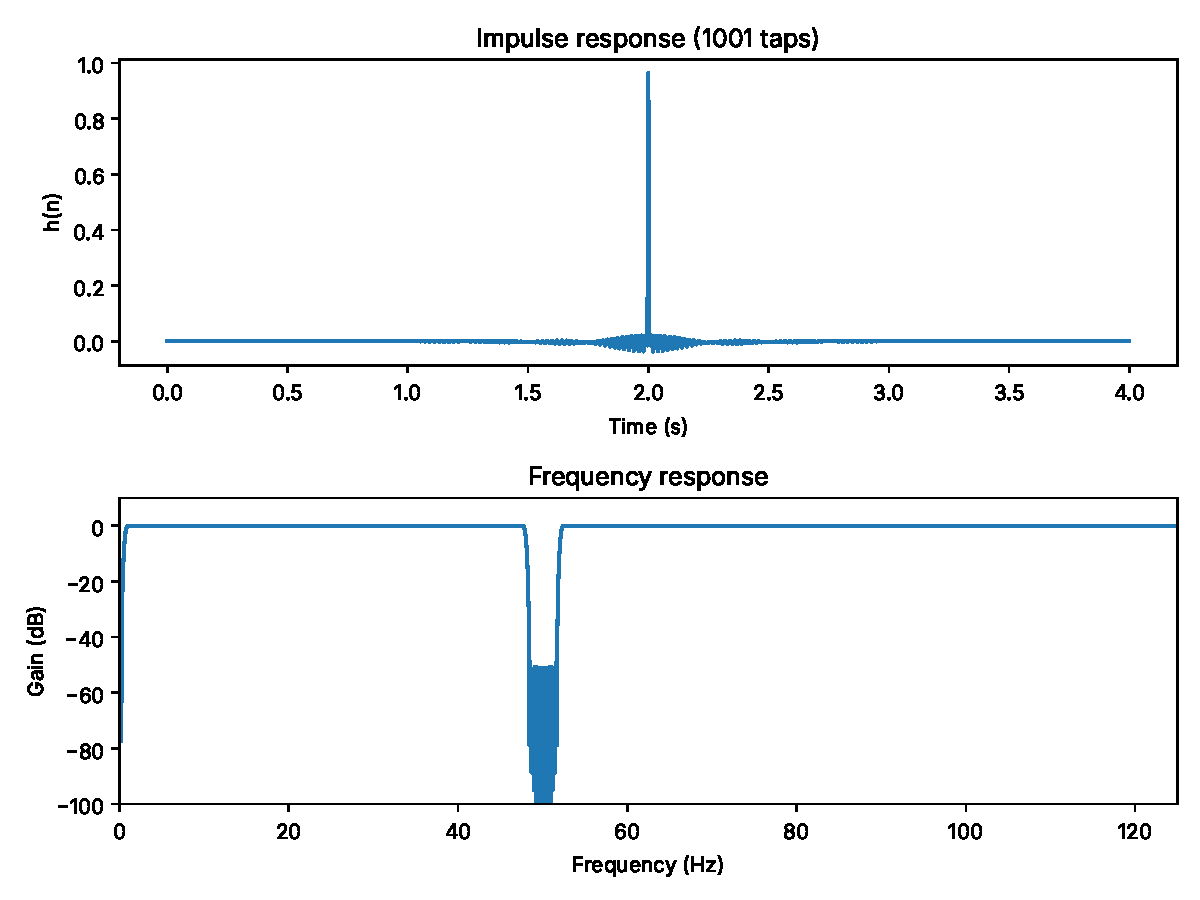
\includegraphics[width=0.72\linewidth]{fir_design.pdf}
  \caption{Designed filter: impulse response (top) and frequency response
           (bottom).}
  \label{fig:design}
\end{figure}

\begin{table}[htbp]
  \centering
  \caption{Measured gain of the designed filter (\cref{fig:design}). Between
           \SI{1.2}{\hertz} and \SI{47}{\hertz}, and from \SI{53}{\hertz} up to
           Nyquist, the gain stays within \SI{\pm 0.03}{\decibel}.}
  \label{tab:gain}
  \begin{tabular}{@{}lcccccccc@{}}
    \toprule
    $f$ (Hz) & 0 & 0.25 & 0.5 & 0.72 & 1.0 & 48 & 50.13 & 52 \\
    \midrule
    Gain (dB) & $-82.3$ & $-74.1$ & $-12.7$ & $-3.0$ & $0.0$ & $-3.4$ & $-53.5$ & $-9.5$ \\
    \bottomrule
  \end{tabular}
\end{table}

% =====================================================================
\section*{Task 3: Realtime FIR Filter}
\label{sec:task3}

\texttt{FIRfilter.dofilter(v)} takes one sample and returns one sample,
evaluating
\begin{equation}
  y[n] = \sum_{m=0}^{M-1} h[m]\,x[n-m]
       = \sum_{m=0}^{p} h[m]\,b[p-m] \;+\! \sum_{m=p+1}^{M-1} h[m]\,b[M+p-m],
  \label{eq:ring}
\end{equation}
where $b$ is a ring buffer of length $M$ and $p$ is where the newest sample was
written. Each new sample overwrites the oldest and the offset moves on, so one
value is written per time step and nothing is shifted. Newest first, the delay
line is $b[p],\dots,b[0],b[M-1],\dots,b[p+1]$, which is two continuous slices.
\texttt{halves} splits $h$ at the same point, so the filter is two dot
products. That is 1001 multiplications per sample, or about \num{250000} per
second at \SI{250}{\hertz}, which is easily realtime.

We feed the ECG in one sample at a time. The first $M$ samples
(\SI{4}{\second}) are left out of the plots while the delay line fills.

\paragraph{The ECG is intact.}
The drift of \SI{4.6}{\milli\volt} is gone and the trace now stays between
\SI{-0.33}{\milli\volt} and \SI{0.73}{\milli\volt} (\cref{fig:t3_ecg}). All
five waves are visible in \cref{fig:t3_beat}. Relative to the R peak
(\SI{0.68}{\milli\volt}), the P wave is at \SI{-140}{\milli\second}, Q at
\SI{-60}{\milli\second}, S at \SI{+28}{\milli\second}
(\SI{-0.26}{\milli\volt}) and T at \SI{+256}{\milli\second}
(\SI{0.32}{\milli\volt}). Because the filter has linear phase, every frequency
is delayed by the same 500 samples, so the shape of the beat does not change.
To check this we measured each R wave's height above the level just before it.
Averaged over all 54 beats, the filtered height is \SI{1.2}{\percent} larger
than the raw height, so the QRS amplitude is preserved.

\paragraph{Spectrum.}
The mains line drops from \SI{42.9}{\micro\volt} to \SI{0.09}{\micro\volt} over
the plotted samples, which is \SI{-53}{\decibel} and agrees with
\cref{tab:gain}. Above \SI{53}{\hertz} the filtered curve sits about
\SI{10}{\decibel} below the raw one even though the filter's gain there is
\SI{0}{\decibel}. This is not filtering. The raw floor is spectral leakage from
the drift, since the spectrum treats the record as periodic and the drift
becomes a step at its ends. Removing a straight line from the raw signal takes
its \SIrange{95}{105}{\hertz} median from \SI{-68.3}{\decibel} to
\SI{-78.4}{\decibel}, which matches the filtered \SI{-78.6}{\decibel}.

\begin{figure}[htbp]
  \centering
  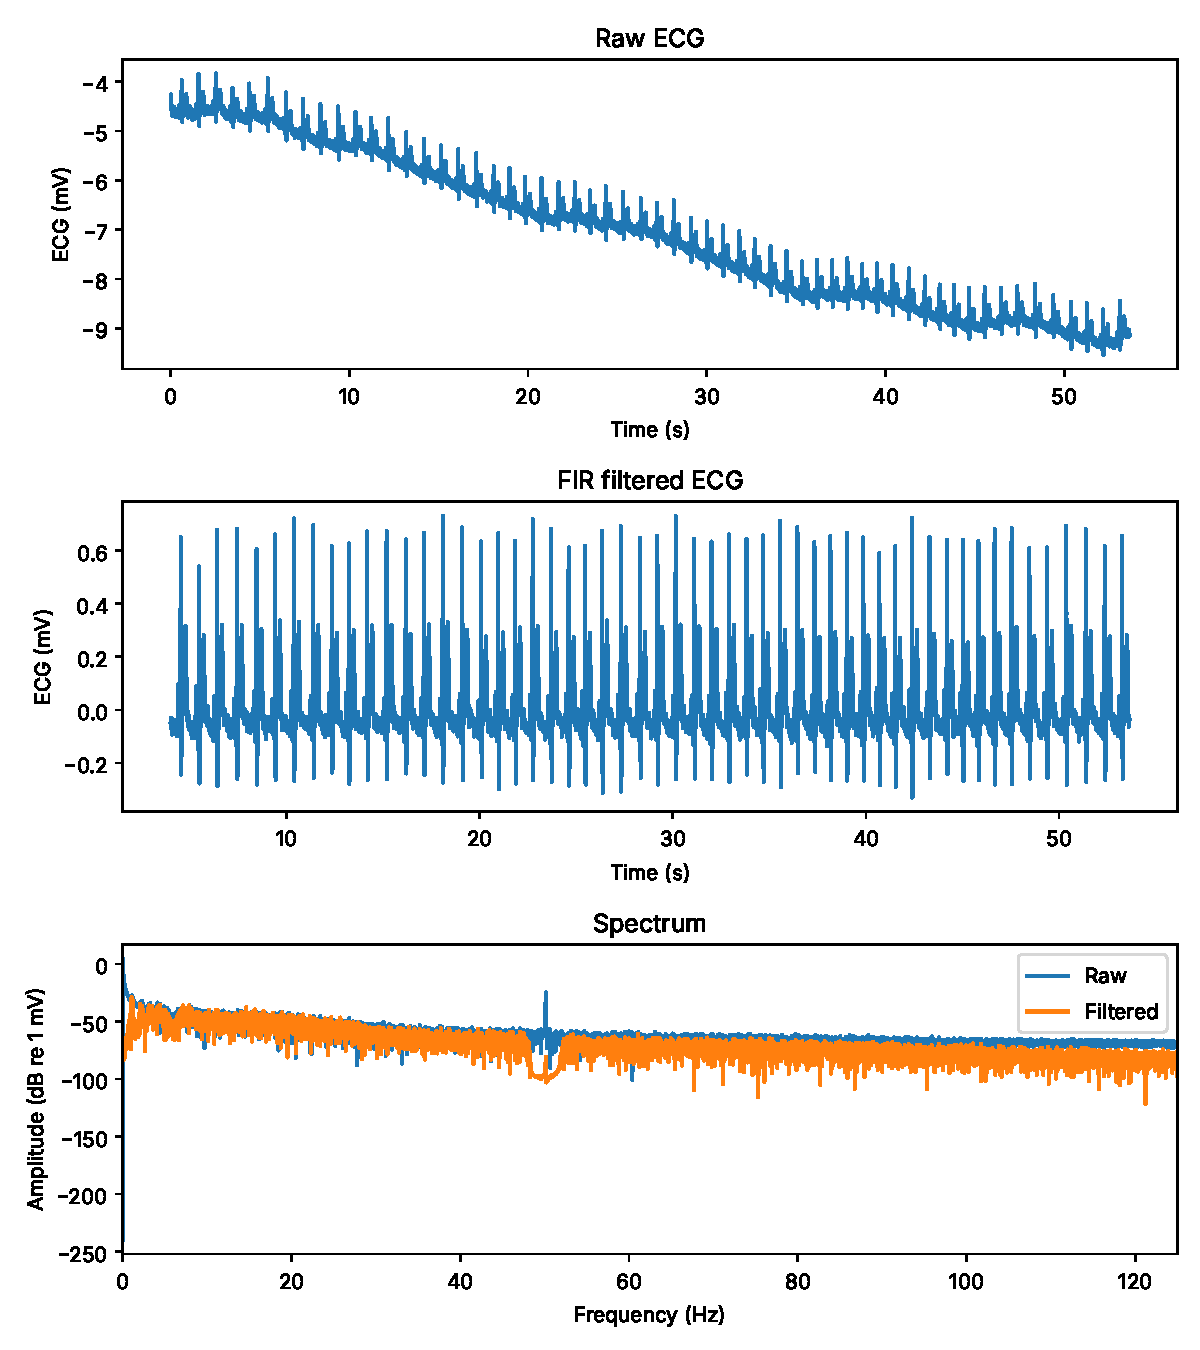
\includegraphics[width=0.74\linewidth]{fir_realtime_ecg.pdf}
  \caption{Patrick's ECG before and after the FIR filter, with the spectra of
           both. The spectra use a dB axis so that the notch is visible.}
  \label{fig:t3_ecg}
\end{figure}

\begin{figure}[htbp]
  \centering
  \begin{tikzpicture}
    \node[anchor=south west,inner sep=0] (im) at (0,0)
      {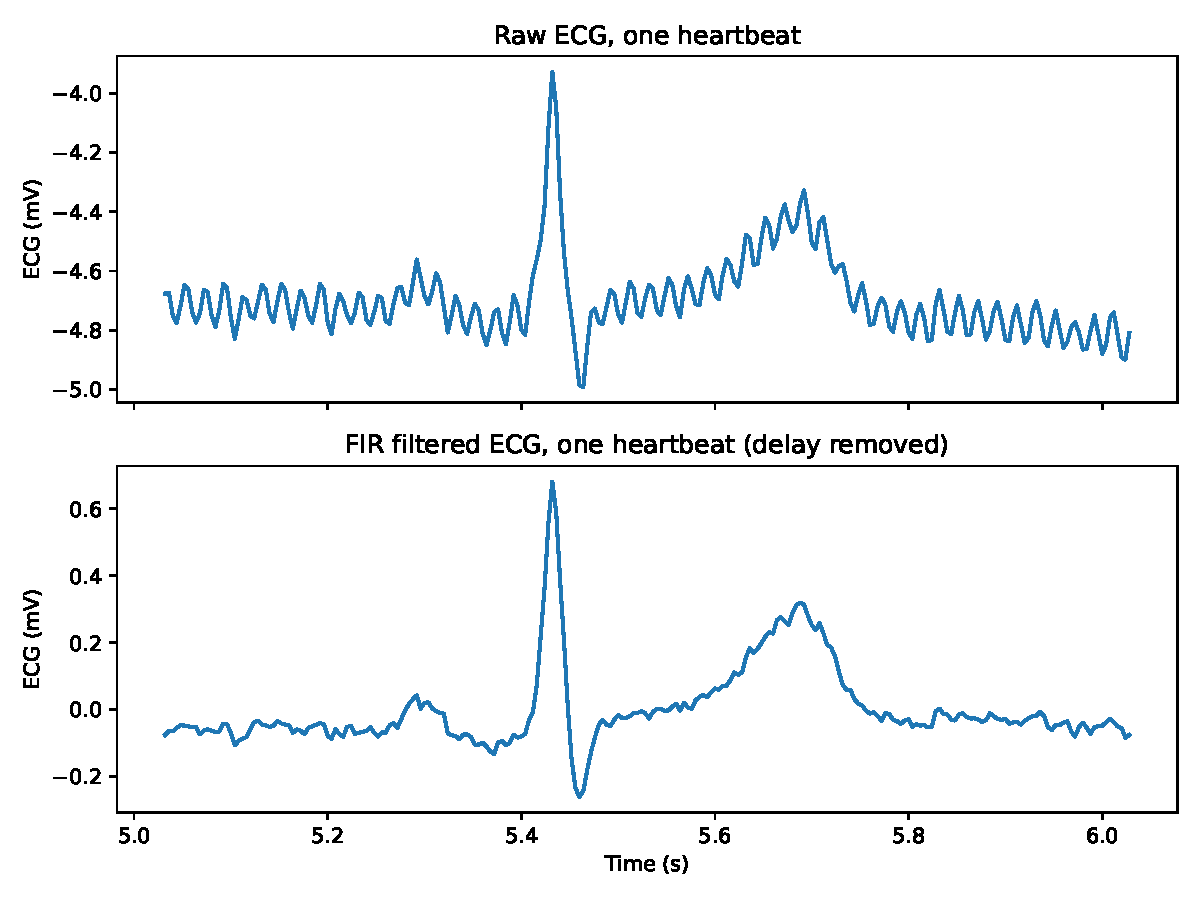
\includegraphics[width=0.74\linewidth]{fir_realtime_beat.pdf}};
    \begin{scope}[x={(im.south east)},y={(im.north west)}]
      \wave{above}{0.3472}{0.2339}{P}
      \wave{below left}{0.4117}{0.1703}{Q}
      \wave{right}{0.4601}{0.4563}{R}
      \wave{below right}{0.4827}{0.1236}{S}
      \wave{above}{0.6667}{0.3348}{T}
    \end{scope}
  \end{tikzpicture}
  \caption{One heartbeat before and after filtering, with the filtered trace
           moved back by the \SI{2.00}{\second} delay so the two line up. The
           PQRST waves are labelled on the filtered trace.}
  \label{fig:t3_beat}
\end{figure}

% =====================================================================
\section*{Task 4: Adaptive LMS Filter}
\label{sec:task4}

\texttt{doFilterAdaptive(signal, noise, learningRate)} also works one sample at
a time. It stores the noise reference in the delay line, subtracts the filter
output from the signal and updates each weight with the LMS rule (lecture
notes, Eq.~147):
\begin{equation}
  e[n] = d[n] - \sum_{m=0}^{M-1} h_m[n]\,x[n-m],
  \qquad
  h_m[n+1] = h_m[n] + \mu\,e[n]\,x[n-m].
  \label{eq:lms}
\end{equation}
The filter can only cancel what is correlated with the reference, so the error
$e[n]$ is the cleaned ECG.

The reference is a sine at the measured mains frequency,
$x[n]=\sin(2\pi\cdot 50.13\,n/f_s)$. It carries no information about baseline
wander, so $d[n]$ is the ECG after a highpass FIR designed with the baseline
band only. That filter also has 1001 taps, so the LMS and bandstop outputs
share the same delay and can be overlaid directly. The LMS has
$f_s/50 = 5$ taps, one mains cycle, which is enough to set the gain and phase
of the sine. We chose $\mu = 0.04$, so that $\mu M P = 0.1$ for a reference
power of $P=\tfrac12$. In our tests the filter became unstable at about
$\mu M P = 2$. Raising $\mu$ below that limit removes more of the mains but
distorts the ECG: at $\mu = 0.2$ the largest R peak grows from
\SI{0.77}{\milli\volt} to \SI{0.88}{\milli\volt}, most likely because the
weights start to react to the QRS complex itself.

\begin{figure}[htbp]
  \centering
  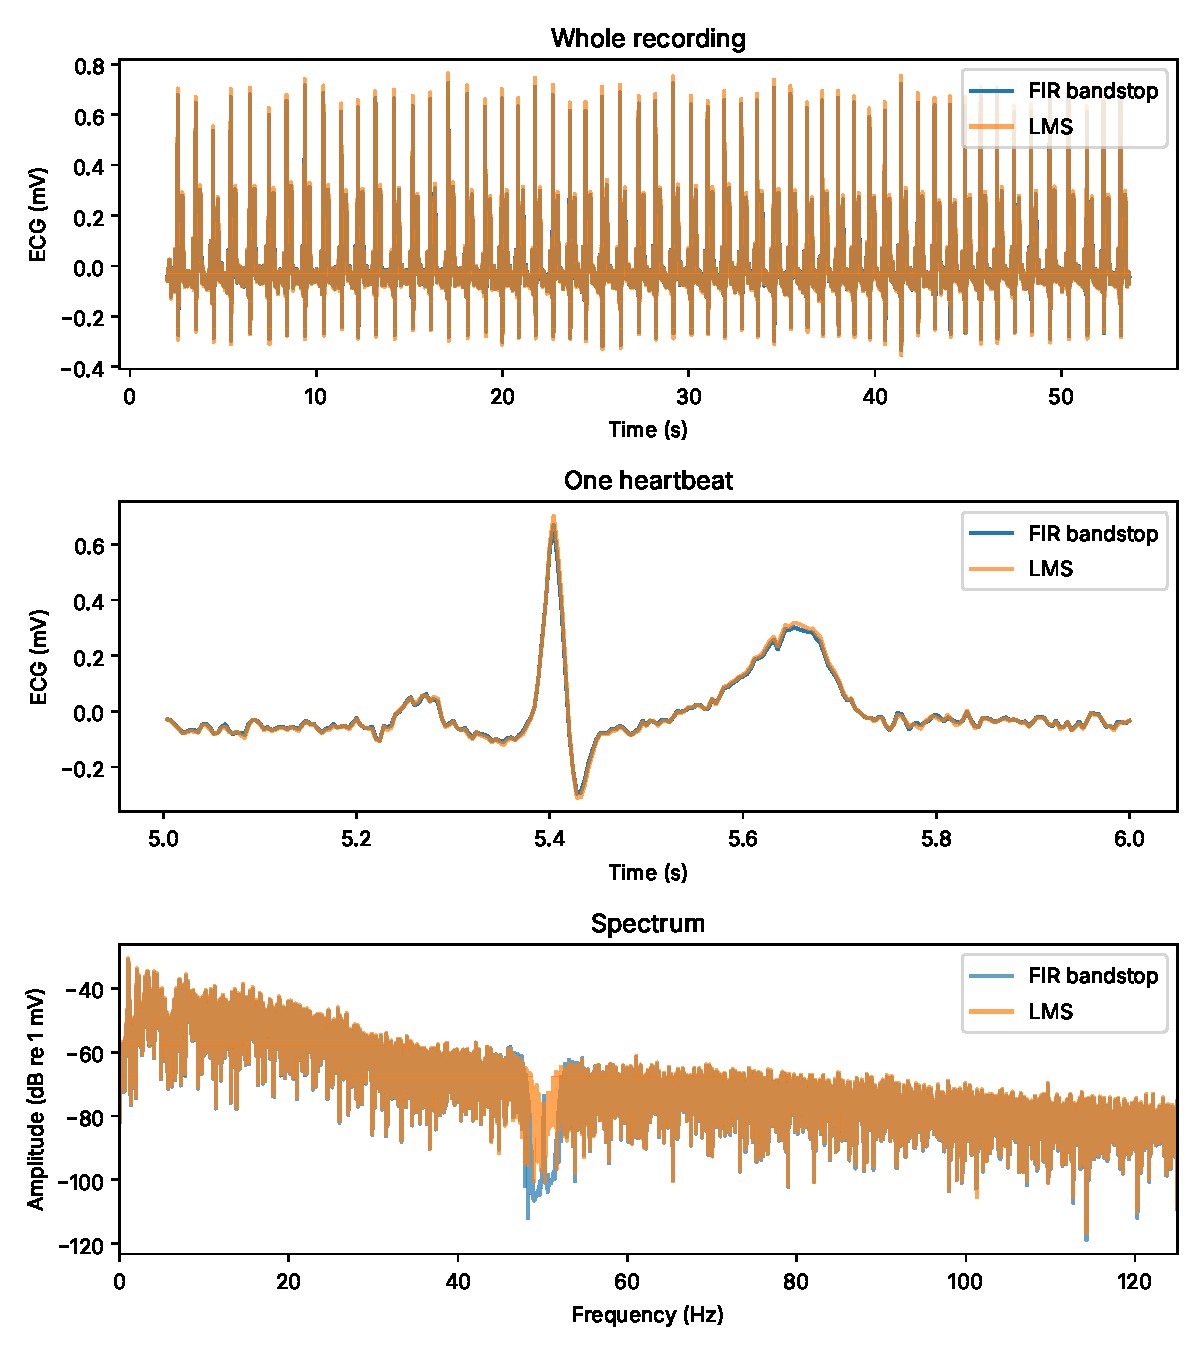
\includegraphics[width=0.74\linewidth]{lms_filter.pdf}
  \caption{FIR bandstop and LMS outputs compared over the whole recording, for
           one heartbeat, and in the frequency domain.}
  \label{fig:lms}
\end{figure}

\begin{table}[htbp]
  \centering
  \caption{FIR bandstop and LMS compared. The mains residual is measured
           against the \SI{43.7}{\micro\volt} left after highpass filtering
           alone.}
  \label{tab:lms}
  \begin{tabular}{@{}lcc@{}}
    \toprule
    & FIR bandstop & LMS \\
    \midrule
    Filters & 1001-tap bandstop & 1001-tap highpass + 5-tap LMS \\
    Delay & \SI{2.00}{\second} & \SI{2.00}{\second} \\
    Multiplications per sample & 1001 & 1011 \\
    Mains residual at \SI{50.13}{\hertz} & \SI{0.09}{\micro\volt} (\SI{-53.4}{\decibel})
      & \SI{0.18}{\micro\volt} (\SI{-47.8}{\decibel}) \\
    Largest value, \SIrange{48}{52}{\hertz} & \SI{0.40}{\micro\volt} & \SI{0.62}{\micro\volt} \\
    Largest R peak & \SI{0.73}{\milli\volt} & \SI{0.77}{\milli\volt} \\
    \bottomrule
  \end{tabular}
\end{table}

The two outputs are almost identical in the time domain (\cref{fig:lms}), with
a correlation of 0.9992 and an RMS difference of \SI{8.3}{\micro\volt}.
\Cref{tab:lms} shows the differences are small. The bandstop goes slightly
deeper at the mains frequency, and in the spectrum its notch is wider because
it removes everything from \SIrange{48}{52}{\hertz}, whereas the LMS only
removes what correlates with the sine. The LMS output has a slightly larger R
peak, for the reason above.

The LMS saves nothing here, since baseline wander still needs the same
1001-tap highpass and therefore the same delay. Its advantage is that it does
not need a fixed band. Even with a reference of exactly \SI{50.00}{\hertz},
\SI{0.13}{\hertz} away from the true mains frequency, the moving weights hold
the residual to \SI{3.0}{\micro\volt}, which is \SI{23}{\decibel} below the
original line. For this recording, where the mains is steady, we would keep
the fixed FIR.

% =====================================================================
\section*{Task 5: Heartbeat Detection}
\label{sec:task5}

The template $r$ is one PQRST of $L=175$ samples (\SI{0.3}{\second} before the
R peak to \SI{0.4}{\second} after) taken from Zabi's FIR-filtered ECG, with its
mean removed. The matched filter is an \texttt{FIRfilter} whose coefficients
are the time-reversed template (lecture notes, Sec.~6.7.10), and its output is
squared so the peaks stand out and the sign does not matter:
\begin{equation}
  h_\text{mf}[n] = r[L-1-n],
  \qquad
  m[n] = \Bigl(\sum_{k=0}^{L-1} h_\text{mf}[k]\,y[n-k]\Bigr)^{2},
  \qquad
  \theta = 0.15\Bigl(\sum_{k} r[k]^2\Bigr)^{2}.
  \label{eq:matched}
\end{equation}
A beat is an upward crossing of the threshold $\theta$. Our first version used
0.3 of the largest output in the whole recording, which a realtime system
cannot know. $\theta$ now comes from the template alone, so it is fixed during
setup, and it found the same 54 beats. The self-match in \cref{eq:matched} is
what the template would give on an identical beat, and the factor of 0.15
allows for Patrick's beats being smaller than Zabi's (R peaks of
\SI{0.7}{\milli\volt} against \SI{1.2}{\milli\volt}). The bandstop, matched
filter, squaring and threshold all run inside one sample-by-sample loop.

The momentary heart rate at beat $i$ is $60 f_s/(b_i-b_{i-1})$, where $b_i$ is
the sample number of the beat. As a heuristic, a crossing less than
$60/200\,f_s = 75$ samples after the last beat would mean a rate above 200 bpm,
so it is treated as noise. The detection itself is dropped rather than just
the rate, so that the interval to the next real beat stays correct.

\begin{figure}[htbp]
  \centering
  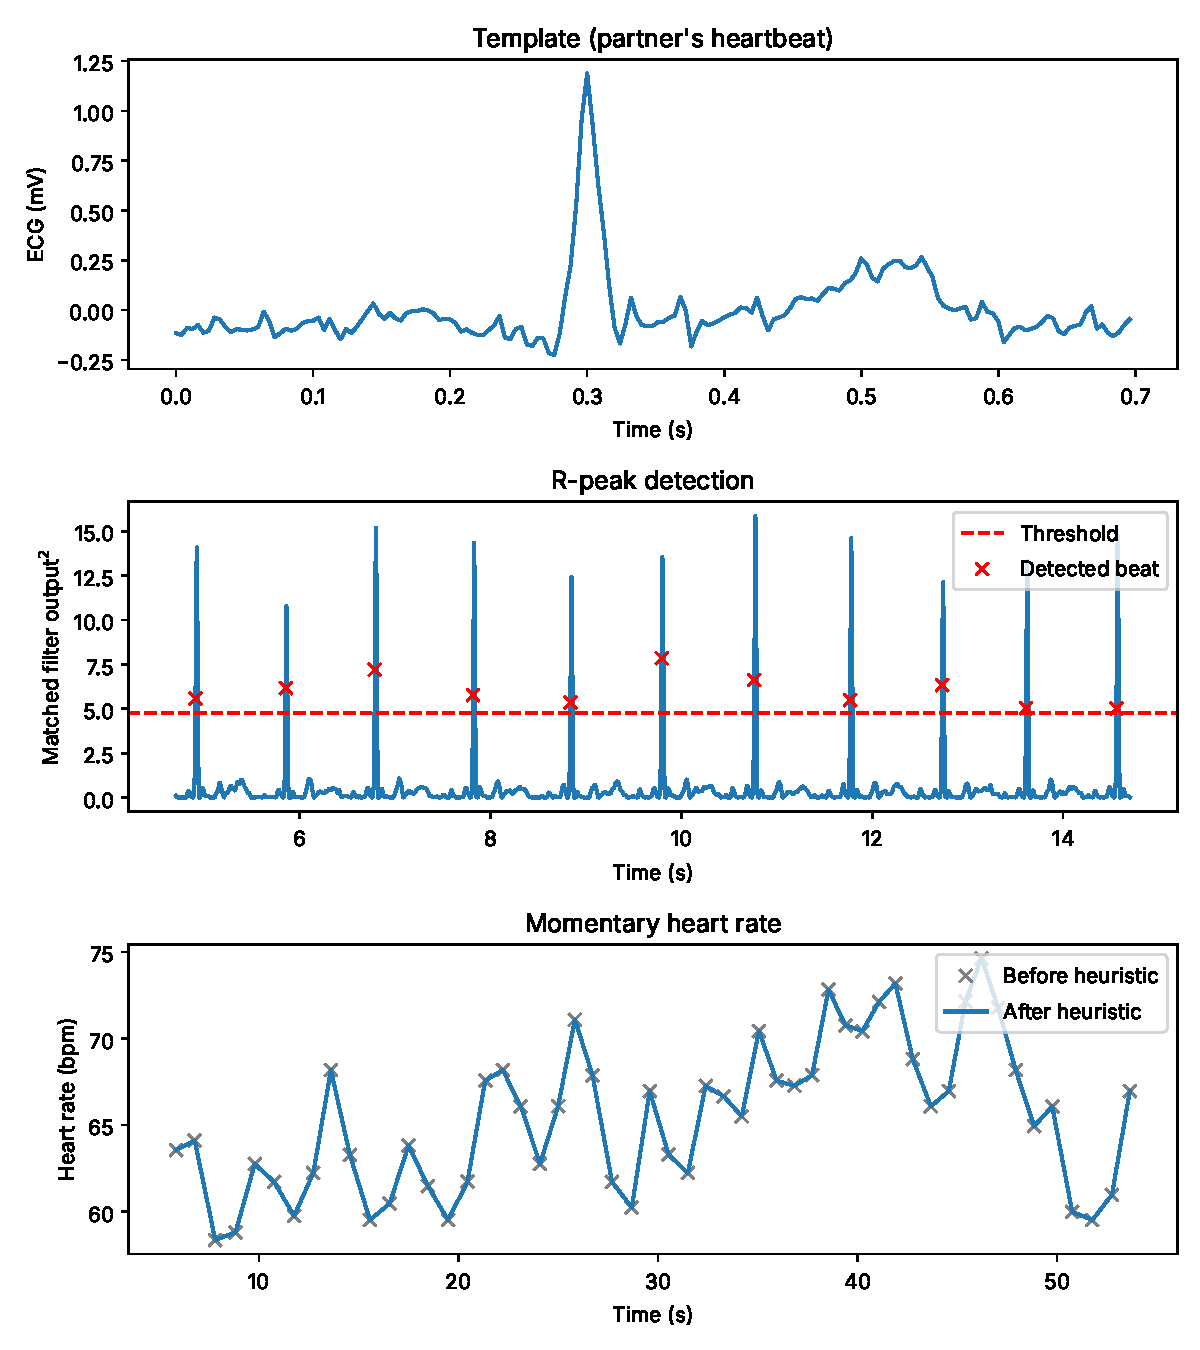
\includegraphics[width=0.74\linewidth]{heartbeat.pdf}
  \caption{The template from Zabi's ECG (top), the squared matched filter
           output on Patrick's ECG for the first \SI{10}{\second} with
           threshold and detections (middle), and the momentary heart rate
           (bottom). No detection was rejected, so the two heart rate curves
           coincide.}
  \label{fig:heartbeat}
\end{figure}

The detector finds all 54 beats, and the heart rate over the 53 intervals runs
from 58.4 to 74.6 bpm with a mean of 65.5 bpm
(\cref{fig:heartbeat}). The heuristic rejected nothing on this recording,
because the margin is wide: the smallest beat peak is 10.7, the threshold is
5.3 and the largest output between beats is 1.2. Using a template from another
person works well, with Patrick's beats reaching \SIrange{30}{45}{\percent} of
the self-match.

To check that the heuristic does work, we lowered the factor from 0.15 to 0.03
so that noise crosses the threshold. That produced 58 crossings, of which 4
were rejected, leaving 54 beats and the same heart rate range. At 0.02 there
are 128 crossings and the heuristic is no longer enough, with rates of up to
188 bpm getting through. It is a safety net and does not replace a sensible
threshold.

% =====================================================================
\section*{Conclusion}
\label{sec:conclusion}

The IFFT design with a Hamming window removes DC, baseline wander and mains
while leaving the PQRST waves intact, with R wave height preserved to within
about \SI{1}{\percent}. The narrow \SI{0.5}{\hertz} baseline band sets the
length of the filter, and the price of keeping the heart rate fundamental
untouched is 1001 taps and a \SI{2}{\second} delay. The ring buffer keeps the
realtime cost to one write and $M$ multiplications per sample. The LMS filter
removes the mains almost as well as the fixed bandstop and can cope with a
reference that is slightly off, but it still needs the FIR highpass and so has
no advantage in delay here. The matched filter with a template from the other
partner and a threshold fixed in advance detects all 54 beats, with no false
detections for the heuristic to remove.

% =====================================================================
\section*{Generative AI Acknowledgement}
\label{sec:genai}

Claude Code (model Claude Opus 5.5, Anthropic, November 2026) was used to draft
the text and LaTeX of this report from our code, figures, commit history and
recordings, and to measure the numbers quoted from them.
\fillin{say whether GenAI was used for the Python code (tool name, version,
publisher, and how it was used), and what you did yourselves, e.g.\ recording
the ECGs, the design decisions, writing and optimising the code, and checking
this report.}

% =====================================================================
\section*{Appendix: Python Code}
\label{app:code}
% Reads the scripts straight from Ass2/ so the listing always matches the code
\newcommand{\codefile}[1]{%
  \subsection*{\texttt{\detokenize{#1}}}
  \IfFileExists{Ass2/#1}{\lstinputlisting{Ass2/#1}}{\lstinputlisting{../Ass2/#1}}}

\codefile{ecg_plot.py}
\codefile{fir_design.py}
\codefile{fir_filter.py}
\codefile{fir_realtime_sim.py}
\codefile{lms_filter.py}
\codefile{heartbeat.py}

\end{document}
